\documentclass[11pt]{beamer}
\usepackage{talk}

\begin{document}

\title{transwarp \\ \vspace{0.2cm} \large A header-only C\texttt{++} library for task concurrency}  
\author{Christian Blume}
\date{May 17, 2017} 

\begin{frame}
\titlepage
\end{frame}


\begin{frame}[fragile]
\frametitle{transwarp drive}
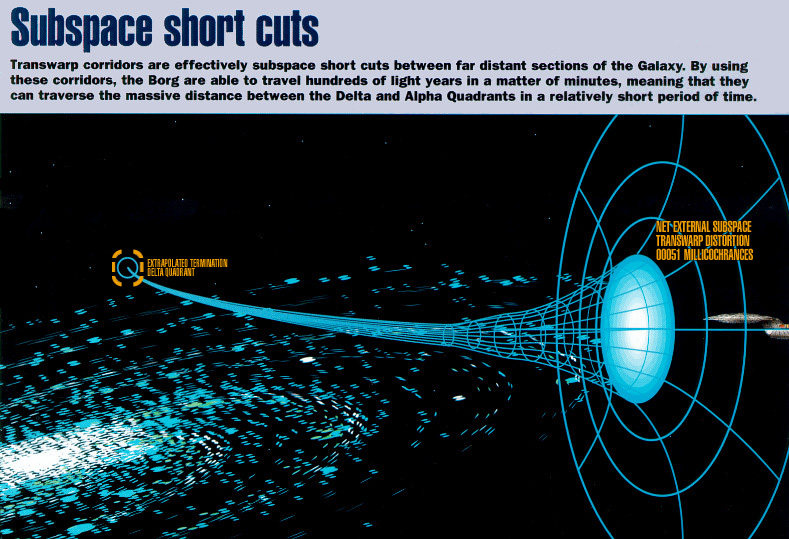
\includegraphics[width=10.8cm]{img/transwarp_conduit.jpg}
\end{frame}


\begin{frame}[fragile]
\frametitle{transwarp library}

A header-only C\texttt{++} library for task concurrency

\bigskip

\url{https://github.com/bloomen/transwarp}

\bigskip
\bigskip

\begin{itemize}
\itemsep 1em
\item Written in C\texttt{++}11 
\item Currently in version 0.1.0
\item Tested using GCC and Clang
\item MIT license
\end{itemize}

\bigskip
\bigskip

Let's chat if you want to contribute!

\end{frame}


\begin{frame}[fragile]
\frametitle{The problem}

\begin{itemize}
\itemsep .5em
\item we have a bunch of operations that depend on each other
\item those operations are run repeatetly with varying input
\item some of those operations are independent
\end{itemize}

\bigskip
\bigskip

Now, we want to:
\bigskip
\begin{itemize}
\itemsep .5em
\item understand the dependencies between operations
\item run the independent operations in parallel
\end{itemize}

\end{frame}


\begin{frame}[fragile]
\frametitle{Typical solution}

\begin{itemize}
\itemsep .5em
\item launch a thread per operation that should run concurrently
\item somehow notify a given operation that it is ready to run
\item collect the results and move on to the next operation
\end{itemize}

\bigskip

Drawbacks
\begin{itemize}
\itemsep .5em
\item explicit thread handling
\item a lot of independent operations may lead to thread contention
\item error prone notification mechanism
\item dependencies are hard to reason about
\end{itemize}

\bigskip

We can do better!

\end{frame}


\begin{frame}[fragile]
\frametitle{Solving it with transwarp}

\begin{itemize}
\itemsep .5em
\item directed acyclic graph of tasks
\item a task can have any number of parent tasks
\item graph must contain a single final task without children
\item underlying thread pool to actually run the tasks
\item a task operation may run anywhere (CPU, GPU, etc)
\end{itemize}

\bigskip
\bigskip

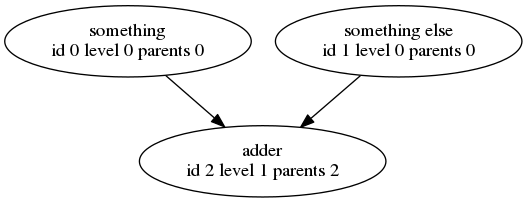
\includegraphics[width=9cm]{img/basic_with_three_tasks.png}

\end{frame}


\begin{frame}[fragile]
\frametitle{Simple example}

\begin{lstlisting}
double add_em_up(double x, int y) {
  return x + y;
}

int main() {
  double value1 = 13.3;
  int value2 = 42;
  auto something = [&value1] { return value1; };
  auto something_else = [&value2] { return value2; };

  auto t1 = make_task("something", something);
  auto t2 = make_task("something else", something_else);
  auto t3 = make_final_task("adder", parallel{4}, add_em_up, t1, t2);

  t3->schedule();
  std::cout << t3->get_future().get(); // 55.3
}
\end{lstlisting}

\end{frame}


\begin{frame}[fragile]
\frametitle{A slightly more evolved example}

\begin{itemize}
\item generate data from a gamma distribution
\item compute statistical measures such as average and median
\item check out the code on github
\end{itemize}

\bigskip

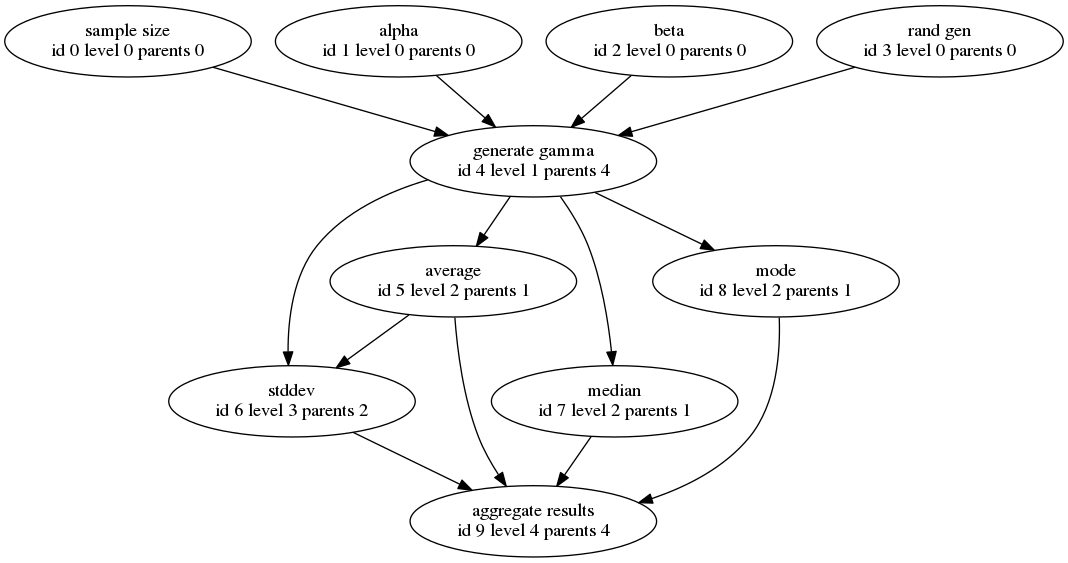
\includegraphics[width=10.8cm]{img/statistical_key_facts.png}
\end{frame}


\begin{frame}[fragile]
\frametitle{The task class}

\begin{lstlisting}
template<typename Functor, typename... Tasks>
class task {
public:

  task(std::string name, Functor functor, 
       std::shared_ptr<Tasks>... parents);

  std::shared_future<result_type> get_future() const;

  const node& get_node() const;

  template<typename Pre, typename Post>
  void visit(Pre& pre_visitor, Post& post_visitor);

  void unvisit();
};
\end{lstlisting}

\end{frame}


\begin{frame}[fragile]
\frametitle{Visiting tasks}
\begin{lstlisting}
template<typename Pre, typename Post>
void task::visit(Pre& pre, Post& post) {
  if (!visited_) {
    pre(*this);
    detail::visit<Pre, Post> visit_task(pre, post);
    detail::call_with_each(visit_task, parents_);
    post(*this);
    visited_ = true;
  }
}

void task::unvisit() {
  if (visited_) {
    visited_ = false;
    detail::call_with_each(detail::unvisit(), parents_);
  }
}
\end{lstlisting}
\end{frame}


\begin{frame}[fragile]
\frametitle{Supporting classes}

\begin{lstlisting}
struct node {
    std::size_t id;
    std::size_t level;
    std::string name;
    std::vector<const node*> parents;
};



struct edge {
    const transwarp::node* child;
    const transwarp::node* parent;
};
\end{lstlisting}

\end{frame}


\begin{frame}[fragile]
\frametitle{The final task class}

\begin{lstlisting}
template<typename Functor, typename... Tasks>
class final_task : public task<Functor, Tasks...> {
public:

  final_task(std::string name, sequenced seq, Functor f, 
             std::shared_ptr<Tasks>... parents);

  final_task(std::string name, parallel par, Functor f, 
             std::shared_ptr<Tasks>... parents);

  void schedule();

  void set_pause(bool enabled);

  void set_cancel(bool enabled);

  const std::vector<edge>& get_graph() const;
};

std::string make_dot(const std::vector<edge>& graph);
\end{lstlisting}

\end{frame}


\begin{frame}[fragile]
\frametitle{Execution policies}
\begin{lstlisting}
class sequenced {};



class parallel {
public:
    parallel(std::size_t n_threads);

    std::size_t n_threads() const;
};
\end{lstlisting}
\end{frame}


\begin{frame}[fragile]
\frametitle{Scheduling tasks}
\begin{lstlisting}
void final_task::schedule() {
  if (!*canceled_) {
    prepare_callbacks();
    if (pool_) { // parallel execution
      for (const auto& callback : callbacks_) {
        pool_->push(callback);
      }
    } else { // sequential execution
      for (const auto& callback : callbacks_) {
        while (paused_) {};
        callback();
      }
    }
  }
}
\end{lstlisting}
\end{frame}


\begin{frame}[fragile]
\frametitle{Creating packagers}
\begin{lstlisting}
detail::wrapped_packager task::make_packager() {
  auto packager = [this] {
    auto futures = detail::get_futures(parents_);
    auto pack_task = std::make_shared<
      std::packaged_task<result_type()>>(std::bind(
      &task::evaluate, std::ref(*this), futures));
    future_ = pack_task->get_future();
    return [pack_task] { (*pack_task)(); };
  };
  return {packager, &node_};
}

static
result_type evaluate(task& t, std::tuple<...> futures) {
  if (*t.canceled_)
    throw task_canceled(t.get_node());
  return detail::call_with_futures<result_type>(
    t.functor_, futures);
}
\end{lstlisting}
\end{frame}


\begin{frame}[fragile]
\frametitle{Scheduling tasks (recap)}
\begin{lstlisting}
void final_task::schedule() {
  if (!*canceled_) {
    prepare_callbacks();
    if (pool_) { // parallel execution
      for (const auto& callback : callbacks_) {
        pool_->push(callback);
      }
    } else { // sequential execution
      for (const auto& callback : callbacks_) {
        while (paused_) {};
        callback();
      }
    }
  }
}
\end{lstlisting}
\end{frame}


\begin{frame}[fragile]
\frametitle{The thread pool}
\begin{lstlisting}
std::queue<std::function<void()>> functors_;
std::condition_variable cond_var_;
std::mutex mutex_;


void thread_pool::push(std::function<void()> func) {
  {
    std::lock_guard<std::mutex> lock(mutex_);
    functors_.push(func);
  }
  cond_var_.notify_one();
}
\end{lstlisting}
\end{frame}


\begin{frame}[fragile]
\frametitle{The thread pool (cont.)}
\begin{lstlisting}
void thread_pool::worker() {
  for (;;) {
    std::function<void()> func;
    {
      std::unique_lock<std::mutex> lock(mutex_);
      cond_var_.wait(lock, [this]{
        return !paused_ && (done_ || !functors_.empty());
      });
      if (done_ && functors_.empty())
        break;
      func = functors_.front();
      functors_.pop();
    }
    func();
  }
}
\end{lstlisting}
\end{frame}


\begin{frame}[fragile]
\frametitle{Summary}

Use transwarp when
\begin{itemize}
\itemsep .5em
\item you have dependent operations
\item the operations are executed repeatetly
\item you consider to run certain operations in parallel
\end{itemize}

\bigskip
\bigskip

What you get is
\begin{itemize}
\itemsep .5em
\item parallelism by design
\item a task graph that is easy to reason about
\item focus on getting stuff done
\end{itemize}

\end{frame}


\begin{frame}[fragile]
\frametitle{Outlook}

\begin{itemize}
\itemsep 1em
\item consider notifications for when futures have been replaced
\item test with C\texttt{++}17 enabled
\item test with Visual Studio
\item add some more real-life examples
\item lift the library to version 1.0
\item \dots
\end{itemize}

\end{frame}


\begin{frame}[fragile]
\huge
Thank You
\end{frame}


\end{document}
